\chapter{Methods in ...}

As manny other  this project developed while its was happening. In this chapter it will be explained what has been done and how it was done. Here is a short summery : 
Set up the Husky with UM7, OS1 and "Point cloud to scan". Then it has all the components needed for Nav2. 
Making husky SLAM, Navigate on pre made map, SLAM and navigation together 
Set up TurtleBot3 with namespace 
To make the TurtleBot3 flow the husky there are multiple options for this: 

\begin{description}
   \item[Mimic] Where the husky and TurtleBot3 resives the same "cmd\_vel" from either telop or Nav2 running on the husky
   \item[Time delay] It is the same as mimic but with a time delay. Husky receives "cmd\_vel" form telop or Nav2. A node called "cmd\_vel\_subpub\_v0.py" also receives "cmd\_vel" converts to tb/cmd\_vel with a time delay witch the TurtleBot3 receives. 
   \item[Nav2 API] Both husky and TurtleBot3 run Nav2, a node receives husky position and sends a "Nav2 Goal" to the TurtleBot3 behind the husky. This can be done with the Nav2 API called "BasicNavigater()" in python.
   \item[AprilTags] The tf between the husky and the TurtleBot3 will be obtained using the AprilTag system. Based on the tf the TurtleBot3 can follow the husky. 
\end{description}


\section{Husky}
\subsection{Hardware}
This section will describe the setup of the Husky and its components. Some of the hardware on the husky has been though changes over time and some don't have. 

The IMU was glued to the center of the tray, connected with a USB to the Xavier. In the Husky there are two Xavier only one of them is used in this project. The other will be referred to as Xavier2. Both of the Xaviers where placed in the tray and secured with a 3D printed mount. The Xaviers where lacking USB ports so both of them got a USB hub. 
The Ouster LiDAR has two components the laser scanner and the power/data brick. The scanner is mounted on top of a aluminum frame in the front for long distance scanning. The brick is blued to the front wall off the tray, connected to 24 volt barrel jack and Ethernet form the ruter. 
The router is mounted in the front of the aluminum frame powered by 12 volt barrel jack. Xavier and Xavier2 is connected with Ethernet, Xavier also has a WiFi connection. 

\subsection{Software}
When setting up the ROS2 software Rviz and rqt was used to test.
Clearpath provides binary packages for the Husky in ROS2 foxy, because of this the hole project was set up foxy. The Clearpath packages provides the essential software for making the husky move with ROS2. This will be referd to as "husky\_base". The "joy\_teleop", "/twist\_mux" and "/huksy\_velocity\_controller". 
"joy\_teleop" converts a Logitech joystick controllers signal into "joy\_teleop/cmd\_vel" a standard velocity massage with namespace. "/twist\_mux" converts "/cmd\_vel" with and without namespaces to "/husky\_velocity\_controller/cmd\_vel\_unstamped" and sends it into "/huksy\_velocity\_controller". Every velocity comand for the Husky goes though the twist node, joystick, keyboard and Nav2. In addition to controlling the motors "/huksy\_velocity\_controller" also publishes "/odom" based on the wheel encounters on the Husky. The "husky\_base" also launches a node called "/ekf\_node" fusing odometry and IMU to localize the Husky. 
An other project on the Husky was pick and place and used the ViperX 300 Robot Arm. This arm was better to set up with Galactic, so the project was converted to Galactic. Foxy and Galactic are similar and didn't cause any issues, except for with the "husky\_base". Clearpath did not provide binary packages for the Husky in Galactic just source. This source files did not initially work on the Husky. The student working on pick and place edited and made some changes to the source files, making them work. Still the source files on Galactic are more unstable then Foxy. "husky\_base" is launched in Foxy and the rest of the project in Galactic. 
The UM7 ROS2 package where found on GitHub. This packages launches a node called "/um7\_dirver" publishing data from the IMU on topic "/imu/data", into "/ekf\_node".
Ouster has a well documented GitHub with ROS2 drivers for there hardware, where the driver for the OS1 was acquired. The package starts up a node called "/ouster\_driver" witch publishes "PoistCloud2" and "/points". Since Nav2 uses "/scan" as perception topic, a packages called "pointcloud\_to\_laserscan" was installed to make the OS1 comunicate with Nav2. 
This image represents software of the Husky in a rqt format where ovals are nodes and squares is topics. 


\section{TurtleBot3}
\subsection{Hardware}
The TurtleBot3 started with no battery and was driven by a Raspberry Pi. The Pi was running Ubuntu Server and had an old student project saved. It had performance issues, writing in the TUI was choppy. The Pi was flashed with Ubuntu Server 20.04 in an attempt to increase the performance. This did not work, and therefor it was decided tho switch out the Pi. A Xavier was available, it is same as the Husky is using and was therefor chosen. The TurtleBot3 uses a battery similar to RC Cars, RC battery's was ordered though a local hobby store. 
%Look at Figure \ref{fig:TB3Hardware}

\begin{figure}[H]
    \centering
    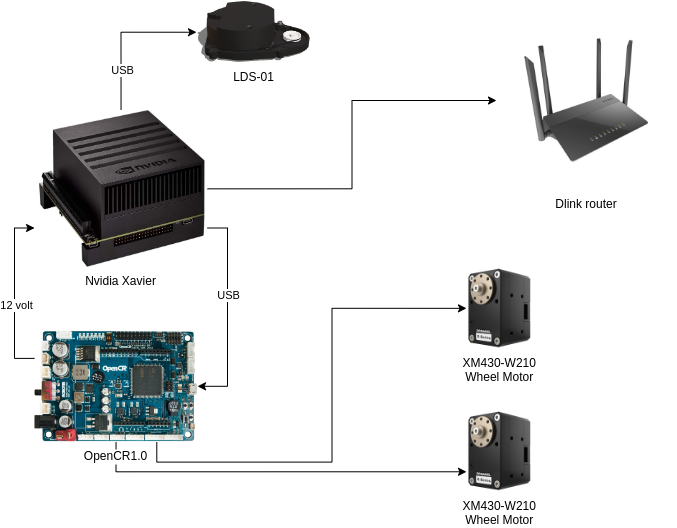
\includegraphics[width = 0.5\textwidth]{Figures/drawio/TB_HW.drawio.png}
    \caption{TurtleBot3 hardware map}
    \label{fig:TB3Hardware}
\end{figure}

\subsection{Software}
The name of user on the TB3 Xavier is tb and will be the reference. tb is running Ubuntu 20.04 Desktop with ROS2 galactic Debian(binary), TB3 packages binary, Nav2 binary. The TB3 packages 